Spatial microsimulation in R: a beginner's guide to iterative
proportional fitting (IPF)

========================================================

\subsection{Introduction}

This document demonstrates how iterative proportional fitting (IPF) can
be performed in R for spatial microsimulation. The aim is to selectively
sample individuals from a survey dataset to fill areas about which only
aggregated values are known. This procedure provides the context for a
paper entitled ``\,`Truncate, replicate, sample': a method for creating
integer weights for spatial microsimulation''.

If you are interested in developing IPF-related algorithms in R, an
updated version of the code is available at the following github
repository: https://github.com/Robinlovelace/IPF-performance-testing .
The aim is to make the IPF code more generalisable, faster and more
compact. Commits/forks welcome.

\subsection{Input data}

Spatial microsimulation requires two input datasets: individual-level
data, where rows represent individuals, and geographically aggregated
data, where rows represent areas. The following code creates example
datasets, based on a survey of 10 individuals and 5 small areas. The
spatial microsimulation model will select individuals based on age, sex
and mode of transport. For consistency with the (larger) model used for
the paper, we will refer to the individual-level data as USd (short for
Understanding Society dataset) and the geographic data as all.msim (all
constraint variables).

\subsubsection{Individual-level data}

\begin{Shaded}
\begin{Highlighting}[]
\CommentTok{# Read in the data in long form (normaly read.table() used)}
\NormalTok{c.names <- }\KeywordTok{c}\NormalTok{(}\StringTok{"id"}\NormalTok{, }\StringTok{"age"}\NormalTok{, }\StringTok{"sex"}\NormalTok{, }\StringTok{"mode"}\NormalTok{)}
\NormalTok{USd <- }\KeywordTok{c}\NormalTok{(       }\DecValTok{1}\NormalTok{, }\DecValTok{27}\NormalTok{, }\StringTok{"m"}\NormalTok{, }\StringTok{"car.d"}\NormalTok{,}
                \DecValTok{2}\NormalTok{, }\DecValTok{54}\NormalTok{, }\StringTok{"m"}\NormalTok{, }\StringTok{"car.d"}\NormalTok{,}
                \DecValTok{3}\NormalTok{, }\DecValTok{35}\NormalTok{, }\StringTok{"f"}\NormalTok{, }\StringTok{"bus"}\NormalTok{,}

                \DecValTok{4}\NormalTok{, }\DecValTok{42}\NormalTok{, }\StringTok{"m"}\NormalTok{, }\StringTok{"walk"}\NormalTok{,}
                \DecValTok{5}\NormalTok{, }\DecValTok{50}\NormalTok{, }\StringTok{"f"}\NormalTok{, }\StringTok{"car.p"}\NormalTok{,}
                \DecValTok{6}\NormalTok{, }\DecValTok{19}\NormalTok{, }\StringTok{"m"}\NormalTok{, }\StringTok{"car.d"}\NormalTok{,}

                \DecValTok{7}\NormalTok{, }\DecValTok{62}\NormalTok{, }\StringTok{"f"}\NormalTok{, }\StringTok{"car.d"}\NormalTok{,}
                \DecValTok{8}\NormalTok{, }\DecValTok{21}\NormalTok{, }\StringTok{"f"}\NormalTok{, }\StringTok{"bicycle"}\NormalTok{,}
                \DecValTok{9}\NormalTok{, }\DecValTok{38}\NormalTok{, }\StringTok{"f"}\NormalTok{, }\StringTok{"walk"}\NormalTok{,}
                \DecValTok{10}\NormalTok{, }\DecValTok{48}\NormalTok{, }\StringTok{"f"}\NormalTok{, }\StringTok{"car.d"}\NormalTok{)}
\NormalTok{USd <- }\KeywordTok{matrix}\NormalTok{(USd, }\DataTypeTok{nrow =} \DecValTok{10}\NormalTok{, }\DataTypeTok{byrow =} \NormalTok{T) }\CommentTok{# Convert long data into matrix, by row}
\NormalTok{USd <- }\KeywordTok{data.frame}\NormalTok{(USd) }\CommentTok{# Convert this into a dataframe}
\KeywordTok{names}\NormalTok{(USd) <- c.names }\CommentTok{# Add correct column names}
\NormalTok{USd$age <- }\KeywordTok{as.numeric}\NormalTok{(}\KeywordTok{levels}\NormalTok{(USd$age)[USd$age]) }\CommentTok{# Age is a numeric variable}

\NormalTok{USd }\CommentTok{# Show the data frame in R}
\end{Highlighting}
\end{Shaded}
\begin{verbatim}
##    id age sex    mode
## 1   1  27   m   car.d
## 2   2  54   m   car.d
## 3   3  35   f     bus
## 4   4  42   m    walk
## 5   5  50   f   car.p
## 6   6  19   m   car.d
## 7   7  62   f   car.d
## 8   8  21   f bicycle
## 9   9  38   f    walk
## 10 10  48   f   car.d
\end{verbatim}
\subsubsection{Geographical data}

\begin{Shaded}
\begin{Highlighting}[]
\CommentTok{# Read in the data in long form (normaly read.table() used)}
\NormalTok{category.labels <- }\KeywordTok{c}\NormalTok{(}\StringTok{"16-30"}\NormalTok{, }\StringTok{"31-50"}\NormalTok{, }\StringTok{"50+"} \CommentTok{# Age constraint }
             \NormalTok{,}\StringTok{"m"}\NormalTok{, }\StringTok{"f"} \CommentTok{# Sex constraint}
             \NormalTok{,}\StringTok{"bicycle"}\NormalTok{, }\StringTok{"bus"}\NormalTok{, }\StringTok{"car.d"}\NormalTok{, }\StringTok{"car.p"}\NormalTok{, }\StringTok{"walk"} \CommentTok{# Mode constraint}
             \NormalTok{)}
\NormalTok{all.msim <- }\KeywordTok{c}\NormalTok{(  }\DecValTok{3}\NormalTok{, }\DecValTok{3}\NormalTok{, }\DecValTok{4}\NormalTok{,   }\DecValTok{5}\NormalTok{, }\DecValTok{5}\NormalTok{,   }\FloatTok{0.001}\NormalTok{, }\DecValTok{1}\NormalTok{, }\DecValTok{8}\NormalTok{, }\DecValTok{1}\NormalTok{, }\FloatTok{0.001}\NormalTok{, }\CommentTok{# Car dominated}
                \DecValTok{2}\NormalTok{, }\DecValTok{2}\NormalTok{, }\DecValTok{6}\NormalTok{,   }\DecValTok{4}\NormalTok{, }\DecValTok{6}\NormalTok{,   }\FloatTok{0.001}\NormalTok{, }\DecValTok{3}\NormalTok{, }\DecValTok{5}\NormalTok{, }\DecValTok{1}\NormalTok{, }\DecValTok{1}\NormalTok{, }\CommentTok{# Elderly}
                \DecValTok{3}\NormalTok{, }\DecValTok{4}\NormalTok{, }\DecValTok{4}\NormalTok{,   }\DecValTok{3}\NormalTok{, }\DecValTok{8}\NormalTok{,   }\DecValTok{1}\NormalTok{, }\DecValTok{2}\NormalTok{, }\DecValTok{5}\NormalTok{, }\DecValTok{2}\NormalTok{, }\DecValTok{1}\NormalTok{, }\CommentTok{# Female dominated}
                \DecValTok{3}\NormalTok{, }\DecValTok{3}\NormalTok{, }\DecValTok{3}\NormalTok{,   }\DecValTok{7}\NormalTok{, }\DecValTok{2}\NormalTok{,   }\DecValTok{2}\NormalTok{, }\DecValTok{1}\NormalTok{, }\DecValTok{3}\NormalTok{, }\DecValTok{1}\NormalTok{, }\DecValTok{2}\NormalTok{, }\CommentTok{# Male dominated}
                \DecValTok{7}\NormalTok{, }\DecValTok{2}\NormalTok{, }\DecValTok{1}\NormalTok{,   }\DecValTok{6}\NormalTok{, }\DecValTok{4}\NormalTok{,   }\DecValTok{7}\NormalTok{, }\FloatTok{0.001}\NormalTok{, }\DecValTok{2}\NormalTok{, }\FloatTok{0.001}\NormalTok{, }\DecValTok{1}  \CommentTok{# Many cyclists, young}
                \NormalTok{)}
\NormalTok{all.msim <- }\KeywordTok{matrix}\NormalTok{(all.msim, }\DataTypeTok{nrow =} \DecValTok{5}\NormalTok{, }\DataTypeTok{byrow =} \NormalTok{T) }\CommentTok{# Convert long data into matrix, by row}
\NormalTok{all.msim <- }\KeywordTok{data.frame}\NormalTok{(all.msim) }\CommentTok{# Convert this into a dataframe}
\KeywordTok{names}\NormalTok{(all.msim) <- category.labels }\CommentTok{# Add correct column names}
\NormalTok{all.msim }\CommentTok{# Show the data frame in R}
\end{Highlighting}
\end{Shaded}
\begin{verbatim}
##   16-30 31-50 50+ m f bicycle   bus car.d car.p  walk
## 1     3     3   4 5 5   0.001 1.000     8 1.000 0.001
## 2     2     2   6 4 6   0.001 3.000     5 1.000 1.000
## 3     3     4   4 3 8   1.000 2.000     5 2.000 1.000
## 4     3     3   3 7 2   2.000 1.000     3 1.000 2.000
## 5     7     2   1 6 4   7.000 0.001     2 0.001 1.000
\end{verbatim}
\begin{Shaded}
\begin{Highlighting}[]

\CommentTok{# Check totals for each constraint match}
\KeywordTok{rowSums}\NormalTok{(all.msim[,}\DecValTok{1}\NormalTok{:}\DecValTok{3}\NormalTok{]) }\CommentTok{# Age constraint}
\end{Highlighting}
\end{Shaded}
\begin{verbatim}
## [1] 10 10 11  9 10
\end{verbatim}
\begin{Shaded}
\begin{Highlighting}[]
\KeywordTok{rowSums}\NormalTok{(all.msim[,}\DecValTok{4}\NormalTok{:}\DecValTok{5}\NormalTok{]) }\CommentTok{# Sex constraint}
\end{Highlighting}
\end{Shaded}
\begin{verbatim}
## [1] 10 10 11  9 10
\end{verbatim}
\begin{Shaded}
\begin{Highlighting}[]
\KeywordTok{rowSums}\NormalTok{(all.msim[,}\DecValTok{6}\NormalTok{:}\DecValTok{10}\NormalTok{])}\CommentTok{# Mode constraint}
\end{Highlighting}
\end{Shaded}
\begin{verbatim}
## [1] 10 10 11  9 10
\end{verbatim}
\subsection{Reweighting the survey dataset}

Iterative proportional fitting will determine the weight allocated to
each individual for each zone to best match the geographically
aggregated data. A weight matrix is therefore created, with rows
corresponding to individuals and columns to zones.

\subsubsection{Create weights: one set of weights for each constraint
and one for starting}

\begin{Shaded}
\begin{Highlighting}[]
\NormalTok{weights0 <- }\KeywordTok{array}\NormalTok{(}\DataTypeTok{dim =} \KeywordTok{c}\NormalTok{(}\KeywordTok{nrow}\NormalTok{(USd), }\KeywordTok{nrow}\NormalTok{(all.msim)))}
\NormalTok{weights1 <- }\KeywordTok{array}\NormalTok{(}\DataTypeTok{dim =} \KeywordTok{c}\NormalTok{(}\KeywordTok{nrow}\NormalTok{(USd), }\KeywordTok{nrow}\NormalTok{(all.msim)))}
\NormalTok{weights2 <- }\KeywordTok{array}\NormalTok{(}\DataTypeTok{dim =} \KeywordTok{c}\NormalTok{(}\KeywordTok{nrow}\NormalTok{(USd), }\KeywordTok{nrow}\NormalTok{(all.msim)))}
\NormalTok{weights3 <- }\KeywordTok{array}\NormalTok{(}\DataTypeTok{dim =} \KeywordTok{c}\NormalTok{(}\KeywordTok{nrow}\NormalTok{(USd), }\KeywordTok{nrow}\NormalTok{(all.msim)))}

\NormalTok{weights0[, ] <- }\DecValTok{1}  \CommentTok{# sets initial weights to 1}
\end{Highlighting}
\end{Shaded}
\subsubsection{Create survey aggregate arrays (for direct comparison
with the geographical aggregate data)}

\begin{Shaded}
\begin{Highlighting}[]
\NormalTok{USd.agg <- }\KeywordTok{array}\NormalTok{(}\DataTypeTok{dim =} \KeywordTok{c}\NormalTok{(}\KeywordTok{nrow}\NormalTok{(all.msim), }\KeywordTok{ncol}\NormalTok{(all.msim)))}
\NormalTok{USd.agg1 <- }\KeywordTok{array}\NormalTok{(}\DataTypeTok{dim =} \KeywordTok{c}\NormalTok{(}\KeywordTok{nrow}\NormalTok{(all.msim), }\KeywordTok{ncol}\NormalTok{(all.msim)))}
\NormalTok{USd.agg2 <- }\KeywordTok{array}\NormalTok{(}\DataTypeTok{dim =} \KeywordTok{c}\NormalTok{(}\KeywordTok{nrow}\NormalTok{(all.msim), }\KeywordTok{ncol}\NormalTok{(all.msim)))}
\NormalTok{USd.agg3 <- }\KeywordTok{array}\NormalTok{(}\DataTypeTok{dim =} \KeywordTok{c}\NormalTok{(}\KeywordTok{nrow}\NormalTok{(all.msim), }\KeywordTok{ncol}\NormalTok{(all.msim)))}
\KeywordTok{colnames}\NormalTok{(USd.agg1) <- category.labels}
\end{Highlighting}
\end{Shaded}
\subsubsection{Convert survey data into wide form}

This step allows the individual-level data to be compared with the
aggregated data directly

\begin{Shaded}
\begin{Highlighting}[]
\NormalTok{USd.cat <- }\KeywordTok{array}\NormalTok{(}\KeywordTok{rep}\NormalTok{(}\DecValTok{0}\NormalTok{), }\DataTypeTok{dim =} \KeywordTok{c}\NormalTok{(}\KeywordTok{nrow}\NormalTok{(USd), }\KeywordTok{length}\NormalTok{(category.labels != }\DecValTok{0}\NormalTok{)))}

\NormalTok{USd.cat[}\KeywordTok{which}\NormalTok{(USd$age <= }\DecValTok{30}\NormalTok{), }\DecValTok{1}\NormalTok{] <- }\DecValTok{1}
\NormalTok{USd.cat[}\KeywordTok{which}\NormalTok{(USd$age >= }\DecValTok{31} \NormalTok{& USd$age <= }\DecValTok{50}\NormalTok{), }\DecValTok{2}\NormalTok{] <- }\DecValTok{1}
\NormalTok{USd.cat[}\KeywordTok{which}\NormalTok{(USd$age > }\DecValTok{50}\NormalTok{), }\DecValTok{3}\NormalTok{] <- }\DecValTok{1}
\NormalTok{USd.cat[}\KeywordTok{which}\NormalTok{(USd$sex == }\StringTok{"m"}\NormalTok{), }\DecValTok{4}\NormalTok{] <- }\DecValTok{1}
\NormalTok{USd.cat[}\KeywordTok{which}\NormalTok{(USd$sex == }\StringTok{"f"}\NormalTok{), }\DecValTok{5}\NormalTok{] <- }\DecValTok{1}
\NormalTok{USd.cat[}\KeywordTok{which}\NormalTok{(USd$mode == }\StringTok{"bicycle"}\NormalTok{), }\DecValTok{6}\NormalTok{] <- }\DecValTok{1}  \CommentTok{# Mode constraints}
\NormalTok{USd.cat[}\KeywordTok{which}\NormalTok{(USd$mode == }\StringTok{"bus"}\NormalTok{), }\DecValTok{7}\NormalTok{] <- }\DecValTok{1}
\NormalTok{USd.cat[}\KeywordTok{which}\NormalTok{(USd$mode == }\StringTok{"car.d"}\NormalTok{), }\DecValTok{8}\NormalTok{] <- }\DecValTok{1}
\NormalTok{USd.cat[}\KeywordTok{which}\NormalTok{(USd$mode == }\StringTok{"car.p"}\NormalTok{), }\DecValTok{9}\NormalTok{] <- }\DecValTok{1}
\NormalTok{USd.cat[}\KeywordTok{which}\NormalTok{(USd$mode == }\StringTok{"walk"}\NormalTok{), }\DecValTok{10}\NormalTok{] <- }\DecValTok{1}
\KeywordTok{sum}\NormalTok{(USd.cat)  }\CommentTok{# Should be 30: 3 variables by 10 individuals}
\end{Highlighting}
\end{Shaded}
\begin{verbatim}
## [1] 30
\end{verbatim}
\begin{Shaded}
\begin{Highlighting}[]

\NormalTok{for (i in }\DecValTok{1}\NormalTok{:}\KeywordTok{nrow}\NormalTok{(all.msim)) \{}
    \CommentTok{# Loop creating aggregate values (to be repeated later)}
    \NormalTok{USd.agg[i, ] <- }\KeywordTok{colSums}\NormalTok{(USd.cat * weights0[, i])}
\NormalTok{\}}

\CommentTok{# Test results}
\NormalTok{USd.agg}
\end{Highlighting}
\end{Shaded}
\begin{verbatim}
##      [,1] [,2] [,3] [,4] [,5] [,6] [,7] [,8] [,9] [,10]
## [1,]    3    5    2    4    6    1    1    5    1     2
## [2,]    3    5    2    4    6    1    1    5    1     2
## [3,]    3    5    2    4    6    1    1    5    1     2
## [4,]    3    5    2    4    6    1    1    5    1     2
## [5,]    3    5    2    4    6    1    1    5    1     2
\end{verbatim}
\begin{Shaded}
\begin{Highlighting}[]
\NormalTok{all.msim}
\end{Highlighting}
\end{Shaded}
\begin{verbatim}
##   16-30 31-50 50+ m f bicycle   bus car.d car.p  walk
## 1     3     3   4 5 5   0.001 1.000     8 1.000 0.001
## 2     2     2   6 4 6   0.001 3.000     5 1.000 1.000
## 3     3     4   4 3 8   1.000 2.000     5 2.000 1.000
## 4     3     3   3 7 2   2.000 1.000     3 1.000 2.000
## 5     7     2   1 6 4   7.000 0.001     2 0.001 1.000
\end{verbatim}
\begin{Shaded}
\begin{Highlighting}[]
\KeywordTok{plot}\NormalTok{(}\KeywordTok{as.vector}\NormalTok{(}\KeywordTok{as.matrix}\NormalTok{(all.msim)), }\KeywordTok{as.vector}\NormalTok{(}\KeywordTok{as.matrix}\NormalTok{(USd.agg)), }\DataTypeTok{xlab =} \StringTok{"Constraints"}\NormalTok{, }
    \DataTypeTok{ylab =} \StringTok{"Model output"}\NormalTok{)}
\KeywordTok{abline}\NormalTok{(}\DataTypeTok{a =} \DecValTok{0}\NormalTok{, }\DataTypeTok{b =} \DecValTok{1}\NormalTok{)}
\end{Highlighting}
\end{Shaded}
\begin{figure}[htbp]
\centering
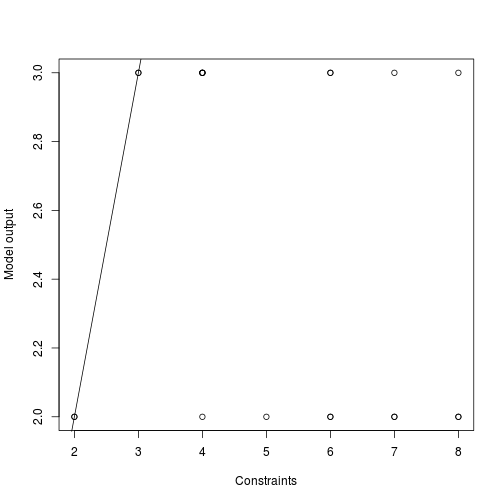
\includegraphics{figure/unnamed-chunk-5.png}
\caption{plot of chunk unnamed-chunk-5}
\end{figure}

\begin{Shaded}
\begin{Highlighting}[]
\KeywordTok{cor}\NormalTok{(}\KeywordTok{as.vector}\NormalTok{(}\KeywordTok{as.matrix}\NormalTok{(all.msim)), }\KeywordTok{as.vector}\NormalTok{(}\KeywordTok{as.matrix}\NormalTok{(USd.agg)))}
\end{Highlighting}
\end{Shaded}
\begin{verbatim}
## [1] 0.546
\end{verbatim}
Note that for USd.agg, the results are the same for every zone, as each
individual has a weight of 1 for every zone. The next stage is to apply
the first constraint, to adjust the weights of each individual so they
match the age constraints.

\subsubsection{Constraint 1: age}

\begin{Shaded}
\begin{Highlighting}[]
\NormalTok{for (j in }\DecValTok{1}\NormalTok{:}\KeywordTok{nrow}\NormalTok{(all.msim)) \{}
    \NormalTok{weights1[}\KeywordTok{which}\NormalTok{(USd$age <= }\DecValTok{30}\NormalTok{), j] <- all.msim[j, }\DecValTok{1}\NormalTok{]/USd.agg[j, }\DecValTok{1}\NormalTok{]}
    \NormalTok{weights1[}\KeywordTok{which}\NormalTok{(USd$age >= }\DecValTok{31} \NormalTok{& USd$age <= }\DecValTok{50}\NormalTok{), j] <- all.msim[j, }\DecValTok{2}\NormalTok{]/USd.agg[j, }
        \DecValTok{2}\NormalTok{]}
    \NormalTok{weights1[}\KeywordTok{which}\NormalTok{(USd$age >= }\DecValTok{51}\NormalTok{), j] <- all.msim[j, }\DecValTok{3}\NormalTok{]/USd.agg[j, }\DecValTok{3}\NormalTok{]  ##}
\NormalTok{\}}
\CommentTok{# Aggregate the results for each zone}
\NormalTok{for (i in }\DecValTok{1}\NormalTok{:}\KeywordTok{nrow}\NormalTok{(all.msim)) \{}
    \NormalTok{USd.agg1[i, ] <- }\KeywordTok{colSums}\NormalTok{(USd.cat * weights0[, i] * weights1[, i])}
\NormalTok{\}}
\CommentTok{# Test results}
\NormalTok{USd.agg1}
\end{Highlighting}
\end{Shaded}
\begin{verbatim}
##      16-30 31-50 50+     m     f bicycle bus car.d car.p walk
## [1,]     3     3   4 4.600 5.400  1.0000 0.6 6.600   0.6  1.2
## [2,]     2     2   6 4.733 5.267  0.6667 0.4 7.733   0.4  0.8
## [3,]     3     4   4 4.800 6.200  1.0000 0.8 6.800   0.8  1.6
## [4,]     3     3   3 4.100 4.900  1.0000 0.6 5.600   0.6  1.2
## [5,]     7     2   1 5.567 4.433  2.3333 0.4 6.067   0.4  0.8
\end{verbatim}
\begin{Shaded}
\begin{Highlighting}[]
\NormalTok{all.msim}
\end{Highlighting}
\end{Shaded}
\begin{verbatim}
##   16-30 31-50 50+ m f bicycle   bus car.d car.p  walk
## 1     3     3   4 5 5   0.001 1.000     8 1.000 0.001
## 2     2     2   6 4 6   0.001 3.000     5 1.000 1.000
## 3     3     4   4 3 8   1.000 2.000     5 2.000 1.000
## 4     3     3   3 7 2   2.000 1.000     3 1.000 2.000
## 5     7     2   1 6 4   7.000 0.001     2 0.001 1.000
\end{verbatim}
\begin{Shaded}
\begin{Highlighting}[]
\KeywordTok{plot}\NormalTok{(}\KeywordTok{as.vector}\NormalTok{(}\KeywordTok{as.matrix}\NormalTok{(all.msim)), }\KeywordTok{as.vector}\NormalTok{(}\KeywordTok{as.matrix}\NormalTok{(USd.agg1)), }\DataTypeTok{xlab =} \StringTok{"Constraints"}\NormalTok{, }
    \DataTypeTok{ylab =} \StringTok{"Model output"}\NormalTok{)}
\KeywordTok{abline}\NormalTok{(}\DataTypeTok{a =} \DecValTok{0}\NormalTok{, }\DataTypeTok{b =} \DecValTok{1}\NormalTok{)}
\end{Highlighting}
\end{Shaded}
\begin{figure}[htbp]
\centering
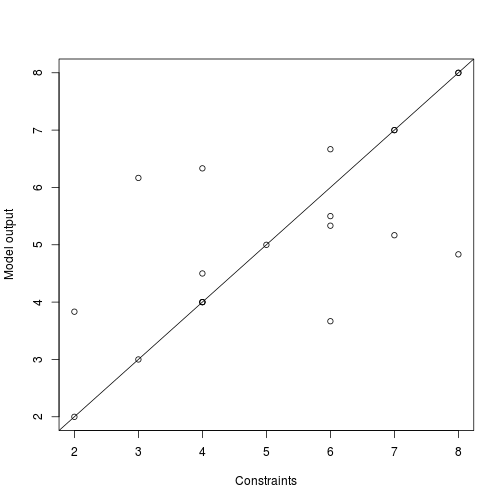
\includegraphics{figure/unnamed-chunk-6.png}
\caption{plot of chunk unnamed-chunk-6}
\end{figure}

\begin{Shaded}
\begin{Highlighting}[]
\KeywordTok{cor}\NormalTok{(}\KeywordTok{as.vector}\NormalTok{(}\KeywordTok{as.matrix}\NormalTok{(all.msim)), }\KeywordTok{as.vector}\NormalTok{(}\KeywordTok{as.matrix}\NormalTok{(USd.agg1)))}
\end{Highlighting}
\end{Shaded}
\begin{verbatim}
## [1] 0.7944
\end{verbatim}
As indicated by the plots and the correlation values, the fit between
the individual-level data and the aggregate constraints (the inpute
data) has been vastly improved, just by constraining by a single
variable. We will perform the test after each constraint to ensure our
model is improving. To see how the weights change for each individual
for each area, type weights1 for constraint 1.

\begin{Shaded}
\begin{Highlighting}[]
\NormalTok{weights1}
\end{Highlighting}
\end{Shaded}
\begin{verbatim}
##       [,1]   [,2] [,3] [,4]  [,5]
##  [1,]  1.0 0.6667  1.0  1.0 2.333
##  [2,]  2.0 3.0000  2.0  1.5 0.500
##  [3,]  0.6 0.4000  0.8  0.6 0.400
##  [4,]  0.6 0.4000  0.8  0.6 0.400
##  [5,]  0.6 0.4000  0.8  0.6 0.400
##  [6,]  1.0 0.6667  1.0  1.0 2.333
##  [7,]  2.0 3.0000  2.0  1.5 0.500
##  [8,]  1.0 0.6667  1.0  1.0 2.333
##  [9,]  0.6 0.4000  0.8  0.6 0.400
## [10,]  0.6 0.4000  0.8  0.6 0.400
\end{verbatim}
\subsubsection{Constraint 2: sex}

\begin{Shaded}
\begin{Highlighting}[]
\NormalTok{for (j in }\DecValTok{1}\NormalTok{:}\KeywordTok{nrow}\NormalTok{(all.msim)) \{}
    \NormalTok{weights2[}\KeywordTok{which}\NormalTok{(USd$sex == }\StringTok{"m"}\NormalTok{), j] <- all.msim[j, }\DecValTok{4}\NormalTok{]/USd.agg1[j, }\DecValTok{4}\NormalTok{]}
    \NormalTok{weights2[}\KeywordTok{which}\NormalTok{(USd$sex == }\StringTok{"f"}\NormalTok{), j] <- all.msim[j, }\DecValTok{5}\NormalTok{]/USd.agg1[j, }\DecValTok{5}\NormalTok{]}
\NormalTok{\}}

\NormalTok{for (i in }\DecValTok{1}\NormalTok{:}\KeywordTok{nrow}\NormalTok{(all.msim)) \{}
    \NormalTok{USd.agg2[i, ] <- }\KeywordTok{colSums}\NormalTok{(USd.cat * weights0[, i] * weights1[, i] * weights2[, }
        \NormalTok{i])}
\NormalTok{\}}
\CommentTok{# Test results}
\NormalTok{USd.agg2}
\end{Highlighting}
\end{Shaded}
\begin{verbatim}
##       [,1]  [,2]  [,3] [,4] [,5]   [,6]   [,7]  [,8]   [,9]  [,10]
## [1,] 3.100 2.874 4.026    5    5 0.9259 0.5556 6.755 0.5556 1.2077
## [2,] 1.886 2.161 5.953    4    6 0.7595 0.4557 7.535 0.4557 0.7937
## [3,] 2.540 4.629 3.831    3    8 1.2903 1.0323 6.113 1.0323 1.5323
## [4,] 3.823 2.004 3.173    7    2 0.4082 0.2449 6.833 0.2449 1.2693
## [5,] 7.135 1.875 0.990    6    4 2.1053 0.3609 6.381 0.3609 0.7920
\end{verbatim}
\begin{Shaded}
\begin{Highlighting}[]
\NormalTok{all.msim}
\end{Highlighting}
\end{Shaded}
\begin{verbatim}
##   16-30 31-50 50+ m f bicycle   bus car.d car.p  walk
## 1     3     3   4 5 5   0.001 1.000     8 1.000 0.001
## 2     2     2   6 4 6   0.001 3.000     5 1.000 1.000
## 3     3     4   4 3 8   1.000 2.000     5 2.000 1.000
## 4     3     3   3 7 2   2.000 1.000     3 1.000 2.000
## 5     7     2   1 6 4   7.000 0.001     2 0.001 1.000
\end{verbatim}
\begin{Shaded}
\begin{Highlighting}[]
\KeywordTok{plot}\NormalTok{(}\KeywordTok{as.vector}\NormalTok{(}\KeywordTok{as.matrix}\NormalTok{(all.msim)), }\KeywordTok{as.vector}\NormalTok{(}\KeywordTok{as.matrix}\NormalTok{(USd.agg2)), }\DataTypeTok{xlab =} \StringTok{"Constraints"}\NormalTok{, }
    \DataTypeTok{ylab =} \StringTok{"Model output"}\NormalTok{)}
\KeywordTok{abline}\NormalTok{(}\DataTypeTok{a =} \DecValTok{0}\NormalTok{, }\DataTypeTok{b =} \DecValTok{1}\NormalTok{)}
\end{Highlighting}
\end{Shaded}
\begin{figure}[htbp]
\centering
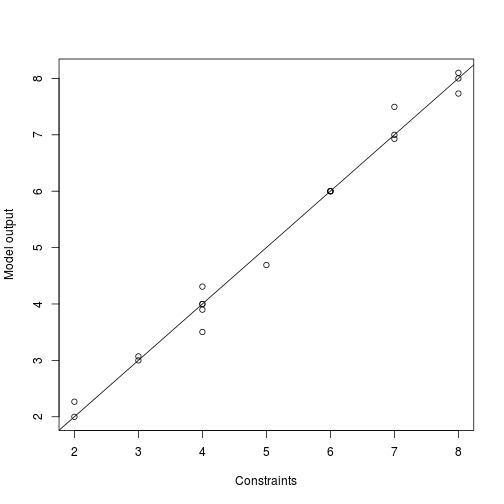
\includegraphics{figure/unnamed-chunk-8.png}
\caption{plot of chunk unnamed-chunk-8}
\end{figure}

\begin{Shaded}
\begin{Highlighting}[]
\KeywordTok{cor}\NormalTok{(}\KeywordTok{as.vector}\NormalTok{(}\KeywordTok{as.matrix}\NormalTok{(all.msim)), }\KeywordTok{as.vector}\NormalTok{(}\KeywordTok{as.matrix}\NormalTok{(USd.agg2)))}
\end{Highlighting}
\end{Shaded}
\begin{verbatim}
## [1] 0.8362
\end{verbatim}
Again the correlation has improved. Now onto the 3rd constraint

\subsubsection{Constraint 3: mode}

\begin{Shaded}
\begin{Highlighting}[]
\NormalTok{for (j in }\DecValTok{1}\NormalTok{:}\KeywordTok{nrow}\NormalTok{(all.msim)) \{}
    \NormalTok{weights3[}\KeywordTok{which}\NormalTok{(USd$mode == }\StringTok{"bicycle"}\NormalTok{), j] <- all.msim[j, }\DecValTok{6}\NormalTok{]/USd.agg2[j, }
        \DecValTok{6}\NormalTok{]}
    \NormalTok{weights3[}\KeywordTok{which}\NormalTok{(USd$mode == }\StringTok{"bus"}\NormalTok{), j] <- all.msim[j, }\DecValTok{7}\NormalTok{]/USd.agg2[j, }\DecValTok{7}\NormalTok{]}
    \NormalTok{weights3[}\KeywordTok{which}\NormalTok{(USd$mode == }\StringTok{"car.d"}\NormalTok{), j] <- all.msim[j, }\DecValTok{8}\NormalTok{]/USd.agg2[j, }\DecValTok{8}\NormalTok{]}
    \NormalTok{weights3[}\KeywordTok{which}\NormalTok{(USd$mode == }\StringTok{"car.p"}\NormalTok{), j] <- all.msim[j, }\DecValTok{9}\NormalTok{]/USd.agg2[j, }\DecValTok{9}\NormalTok{]}
    \NormalTok{weights3[}\KeywordTok{which}\NormalTok{(USd$mode == }\StringTok{"walk"}\NormalTok{), j] <- all.msim[j, }\DecValTok{10}\NormalTok{]/USd.agg2[j, }\DecValTok{10}\NormalTok{]}
\NormalTok{\}}
\NormalTok{weights4 <- weights0 * weights1 * weights2 * weights3}
\NormalTok{for (i in }\DecValTok{1}\NormalTok{:}\KeywordTok{nrow}\NormalTok{(all.msim)) \{}
    \NormalTok{USd.agg3[i, ] <- }\KeywordTok{colSums}\NormalTok{(USd.cat * weights4[, i])}
\NormalTok{\}}
\CommentTok{# Test results}
\NormalTok{USd.agg3}
\end{Highlighting}
\end{Shaded}
\begin{verbatim}
##        [,1]  [,2]   [,3]  [,4]  [,5]  [,6]  [,7] [,8]  [,9] [,10]
## [1,] 2.5755 2.659 4.7676 5.150 4.852 0.001 1.000    8 1.000 0.001
## [2,] 0.7486 5.302 3.9500 2.856 7.145 0.001 3.000    5 1.000 1.000
## [3,] 2.0224 5.844 3.1332 2.371 8.629 1.000 2.000    5 2.000 1.000
## [4,] 3.4992 4.108 1.3932 4.238 4.762 2.000 1.000    3 1.000 2.000
## [5,] 8.5766 1.115 0.3103 2.290 7.712 7.000 0.001    2 0.001 1.000
\end{verbatim}
\begin{Shaded}
\begin{Highlighting}[]
\NormalTok{all.msim}
\end{Highlighting}
\end{Shaded}
\begin{verbatim}
##   16-30 31-50 50+ m f bicycle   bus car.d car.p  walk
## 1     3     3   4 5 5   0.001 1.000     8 1.000 0.001
## 2     2     2   6 4 6   0.001 3.000     5 1.000 1.000
## 3     3     4   4 3 8   1.000 2.000     5 2.000 1.000
## 4     3     3   3 7 2   2.000 1.000     3 1.000 2.000
## 5     7     2   1 6 4   7.000 0.001     2 0.001 1.000
\end{verbatim}
\begin{Shaded}
\begin{Highlighting}[]
\KeywordTok{plot}\NormalTok{(}\KeywordTok{as.vector}\NormalTok{(}\KeywordTok{as.matrix}\NormalTok{(all.msim)), }\KeywordTok{as.vector}\NormalTok{(}\KeywordTok{as.matrix}\NormalTok{(USd.agg3)), }\DataTypeTok{xlab =} \StringTok{"Constraints"}\NormalTok{, }
    \DataTypeTok{ylab =} \StringTok{"Model output"}\NormalTok{)}
\KeywordTok{abline}\NormalTok{(}\DataTypeTok{a =} \DecValTok{0}\NormalTok{, }\DataTypeTok{b =} \DecValTok{1}\NormalTok{)}
\end{Highlighting}
\end{Shaded}
\begin{figure}[htbp]
\centering
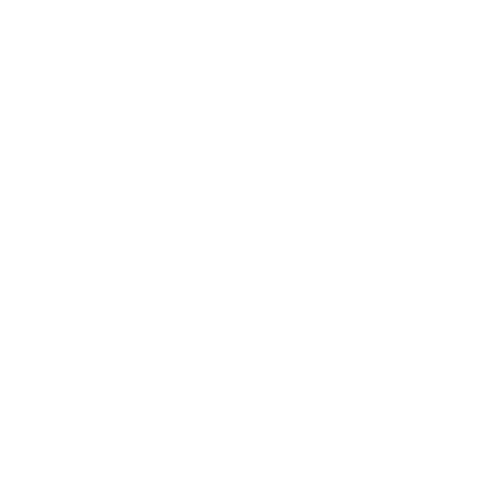
\includegraphics{figure/unnamed-chunk-9.png}
\caption{plot of chunk unnamed-chunk-9}
\end{figure}

\begin{Shaded}
\begin{Highlighting}[]
\KeywordTok{cor}\NormalTok{(}\KeywordTok{as.vector}\NormalTok{(}\KeywordTok{as.matrix}\NormalTok{(all.msim)), }\KeywordTok{as.vector}\NormalTok{(}\KeywordTok{as.matrix}\NormalTok{(USd.agg3)))}
\end{Highlighting}
\end{Shaded}
\begin{verbatim}
## [1] 0.8588
\end{verbatim}
\begin{Shaded}
\begin{Highlighting}[]
\KeywordTok{rowSums}\NormalTok{(USd.agg3[, }\DecValTok{1}\NormalTok{:}\DecValTok{3}\NormalTok{])  }\CommentTok{# The total population modelled for each zone, constraint 1}
\end{Highlighting}
\end{Shaded}
\begin{verbatim}
## [1] 10 10 11  9 10
\end{verbatim}
\begin{Shaded}
\begin{Highlighting}[]
\KeywordTok{rowSums}\NormalTok{(USd.agg3[, }\DecValTok{4}\NormalTok{:}\DecValTok{5}\NormalTok{])}
\end{Highlighting}
\end{Shaded}
\begin{verbatim}
## [1] 10 10 11  9 10
\end{verbatim}
\begin{Shaded}
\begin{Highlighting}[]
\KeywordTok{rowSums}\NormalTok{(USd.agg3[, }\DecValTok{6}\NormalTok{:}\DecValTok{10}\NormalTok{])}
\end{Highlighting}
\end{Shaded}
\begin{verbatim}
## [1] 10 10 11  9 10
\end{verbatim}
\subsection{Iterations}

The correlation has been improved from one constraint to the next. Even
the after the final constraint (mode), which differs greatly from the
survey data for some zones, the correlation has improved. This
illustrates the robustness of the IPF method. Also note that the
population of each simulated zone is correct. The next step is to
perform further iterations, using the results of the first iteration
(weights4) as our starting point.

\begin{Shaded}
\begin{Highlighting}[]
\NormalTok{weights0 <- weights4}
\NormalTok{USd.agg}\FloatTok{.1} \NormalTok{<- USd.agg  }\CommentTok{# Saving this for future reference}
\end{Highlighting}
\end{Shaded}
After running this command, simply run the model again, beginning from
the loop at the end of the R code section titled ``Convert survey data
into wide form''. After running constraint 3 the second time, the
correlation is higher: 0.89 instead of 0.86 . Because this is a
relatively simple example, the fit between constraint and simulated
aggregate variables will not improve much beyond this point (notice the
similarity between the plot below - of the final result after the 2nd
iteration - and the plot above).

After the second iteration, the results are as follows:

\begin{Shaded}
\begin{Highlighting}[]
\KeywordTok{plot}\NormalTok{(}\KeywordTok{as.vector}\NormalTok{(}\KeywordTok{as.matrix}\NormalTok{(all.msim)), }\KeywordTok{as.vector}\NormalTok{(}\KeywordTok{as.matrix}\NormalTok{(USd.agg3)), }\DataTypeTok{xlab =} \StringTok{"Constraints"}\NormalTok{, }
    \DataTypeTok{ylab =} \StringTok{"Model output"}\NormalTok{)}
\KeywordTok{abline}\NormalTok{(}\DataTypeTok{a =} \DecValTok{0}\NormalTok{, }\DataTypeTok{b =} \DecValTok{1}\NormalTok{)}
\end{Highlighting}
\end{Shaded}
\begin{figure}[htbp]
\centering
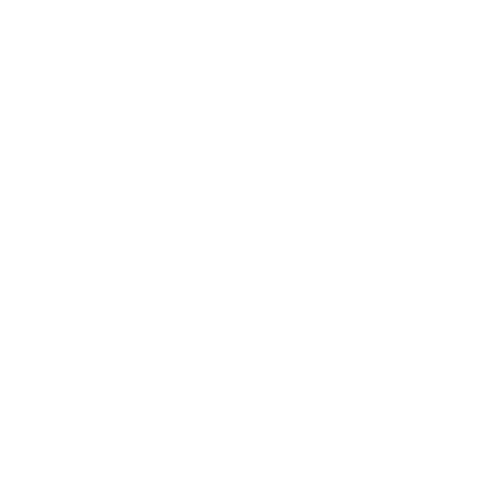
\includegraphics{figure/unnamed-chunk-12.png}
\caption{plot of chunk unnamed-chunk-12}
\end{figure}

\begin{Shaded}
\begin{Highlighting}[]
\KeywordTok{cor}\NormalTok{(}\KeywordTok{as.vector}\NormalTok{(}\KeywordTok{as.matrix}\NormalTok{(all.msim)), }\KeywordTok{as.vector}\NormalTok{(}\KeywordTok{as.matrix}\NormalTok{(USd.agg3)))}
\end{Highlighting}
\end{Shaded}
\begin{verbatim}
## [1] 0.8847
\end{verbatim}
\subsection{Interrogating the results}

To view the characteristics of representative individuals for each zone,
the vector associated with the zone in question can be called from the
final weight matrix (weights4 in this case). The individuals that best
match (have the highest weights) for zone five for example, which
contains a high proportion of young cyclists, can be viewed with the
following command:

\begin{Shaded}
\begin{Highlighting}[]
\KeywordTok{cbind}\NormalTok{(weights4[, }\DecValTok{5}\NormalTok{], USd)}
\end{Highlighting}
\end{Shaded}
\begin{verbatim}
##    weights4[, 5] id age sex    mode
## 1        0.64259  1  27   m   car.d
## 2        0.54367  2  54   m   car.d
## 3        0.00100  3  35   f     bus
## 4        0.82114  4  42   m    walk
## 5        0.00100  5  50   f   car.p
## 6        0.64259  6  19   m   car.d
## 7        0.11842  7  62   f   car.d
## 8        7.00000  8  21   f bicycle
## 9        0.17886  9  38   f    walk
## 10       0.05273 10  48   f   car.d
\end{verbatim}
The output from this command illustrates why the final solution of the
IPF procedure is not perfect (i.e.~why the correlation between the
constraint and simulated aggregates cannot be 1): there is only 1
cyclist in the sample population, so she must be replicated 7 times to
fulfill the number of cyclists in the constraint variables, distorting
the other results. This example demonstrates the importance of having a
large and diverse survey dataset from which individuals can be sampled.

For some areas the results are better than others. A breakdown of model
fit by area can be seen by recursively running the correlation command:

\begin{Shaded}
\begin{Highlighting}[]
\NormalTok{for (i in }\DecValTok{1}\NormalTok{:}\KeywordTok{nrow}\NormalTok{(all.msim)) \{}
    \NormalTok{all.msim$cor[i] <- }\KeywordTok{cor}\NormalTok{(}\KeywordTok{as.vector}\NormalTok{(}\KeywordTok{as.matrix}\NormalTok{(all.msim[i, }\DecValTok{1}\NormalTok{:}\DecValTok{10}\NormalTok{])), USd.agg3[i, }
        \NormalTok{])}
\NormalTok{\}}
\NormalTok{all.msim}
\end{Highlighting}
\end{Shaded}
\begin{verbatim}
##   16-30 31-50 50+ m f bicycle   bus car.d car.p  walk    cor
## 1     3     3   4 5 5   0.001 1.000     8 1.000 0.001 0.9987
## 2     2     2   6 4 6   0.001 3.000     5 1.000 1.000 0.8016
## 3     3     4   4 3 8   1.000 2.000     5 2.000 1.000 0.9648
## 4     3     3   3 7 2   2.000 1.000     3 1.000 2.000 0.7160
## 5     7     2   1 6 4   7.000 0.001     2 0.001 1.000 0.8580
\end{verbatim}
Note that zones 1 and 3 are simulated well. This can be explained
because their attributes already fitted with those of original dataset
well:

\begin{Shaded}
\begin{Highlighting}[]
\NormalTok{for (i in }\DecValTok{1}\NormalTok{:}\KeywordTok{nrow}\NormalTok{(all.msim)) \{}
    \NormalTok{all.msim$cor[i] <- }\KeywordTok{cor}\NormalTok{(}\KeywordTok{as.vector}\NormalTok{(}\KeywordTok{as.matrix}\NormalTok{(all.msim[i, }\DecValTok{1}\NormalTok{:}\DecValTok{10}\NormalTok{])), USd.agg}\FloatTok{.1}\NormalTok{[i, }
        \NormalTok{])}
\NormalTok{\}}
\NormalTok{all.msim}
\end{Highlighting}
\end{Shaded}
\begin{verbatim}
##   16-30 31-50 50+ m f bicycle   bus car.d car.p  walk    cor
## 1     3     3   4 5 5   0.001 1.000     8 1.000 0.001 0.7759
## 2     2     2   6 4 6   0.001 3.000     5 1.000 1.000 0.5728
## 3     3     4   4 3 8   1.000 2.000     5 2.000 1.000 0.8375
## 4     3     3   3 7 2   2.000 1.000     3 1.000 2.000 0.4152
## 5     7     2   1 6 4   7.000 0.001     2 0.001 1.000 0.2112
\end{verbatim}
\begin{Shaded}
\begin{Highlighting}[]
\NormalTok{USd.agg}\FloatTok{.1}
\end{Highlighting}
\end{Shaded}
\begin{verbatim}
##      [,1] [,2] [,3] [,4] [,5] [,6] [,7] [,8] [,9] [,10]
## [1,]    3    5    2    4    6    1    1    5    1     2
## [2,]    3    5    2    4    6    1    1    5    1     2
## [3,]    3    5    2    4    6    1    1    5    1     2
## [4,]    3    5    2    4    6    1    1    5    1     2
## [5,]    3    5    2    4    6    1    1    5    1     2
\end{verbatim}
This illustrates the importance of using a sample survey dataset that is
fairly representative of the aggregated constraint table.

\subsection{Taking IPF further}

This document has provided a succinct run-through of the IPF procedure
in R. This simplified example illustrates how the R programming language
is well-suited to the task, with a number of in-built functions to
manipulate and analyse the data. Because R is an object-orientated
programming language with many add-ons and the ability to define new
functions, the capabilities outlined above only scratch the surface of
what is possible. For example, it would be possible to create new
individuals which have the characteristics most needed to improve the
overall model fit. Also, the possibility of grouping individuals into
household units would greatly add to the technique's ability to simulate
reality (many statistics are collected, and many decisions are made, at
the household level). Another `add-on' that would be particularly useful
for IPF would be the ability to `integerise' the results. Methods for
performing integerisation in R are compared in a paper that accompanies
this document.

The advancement of the IPF procedure will depend not only on
application, but understanding of the underlying theory. This topic is
beyond the scope of this practical guide. Some references on the
underlying theory and applications of IPF are provided below:

\subsection{Key references on IPF and spatial microsimultion}

Note: this list is just a starter and is no way comprehensive

\href{http://www.jstor.org/stable/2235722}{Deming, W., 1940}. On a least
squares adjustment of a sampled frequency table when the expected
marginal totals are known. The Annals of Mathematical Statistics.

\href{http://dx.doi.org/10.1111/j.0033-0124.1992.00340.x}{Wong, D.W.S.,
1992}. The Reliability of Using the Iterative Proportional Fitting
Procedure. The Professional Geographer, 44(3), pp.340--348.

\href{http://eprints.whiterose.ac.uk/5029/1/99-3.pdf}{Norman, P., 1999}.
Putting Iterative Proportional Fitting (IPF) on the Researcher's Desk.
School of Geography, University of Leeds.

\href{www.jrf.org.uk/sites/files/jrf/1859352669.pdf}{Ballas, D. et al.,
2005}. Geography matters: simulating the local impacts of national
social policies, Joseph Roundtree Foundation.

\href{http://linkinghub.elsevier.com/retrieve/pii/S0198971512000336}{Hermes,
K. \& Poulsen, M., 2012}. A review of current methods to generate
synthetic spatial microdata using reweighting and future directions.
Computers, Environment and Urban Systems, 36(4), pp.281--290.

\href{http://www.springerlink.com/index/10.1007/s11116-011-9367-4}{Pritchard,
D.R. \& Miller, E.J., 2012}. Advances in population synthesis: fitting
many attributes per agent and fitting to household and person margins
simultaneously. Transportation, 39(3), pp.685--704.
